This is a 1-D problem that consists of a domain with 3 regions of differing
saturation values $\frac{q}{\sigma}$. This is used to test both reaction
terms and source terms.
Table \ref{tab:three_region} summarizes the test parameters.

%-------------------------------------------------------------------------------
\begin{table}[htb]\caption{Three-Region Test Problem Summary}
\label{tab:three_region}
\centering
\begin{tabular}{l l}\toprule
\emph{Parameter} & \emph{Value}\\\midrule
Domain & $\mathcal{D} = (0,1)$\\
Initial Conditions & $u_0(x)=0$\\
Boundary Conditions & $u(x,t)=u_{inc}=1$\\
Direction & $\mathbf{\Omega} = \mathbf{e}_x$\\
Cross Section & $\sigma(\x)=\left\{\begin{array}{c l}
   \sigma_0, & x\in[x_0,x_1]\\
   \sigma_1, & x\in(x_1,x_2]\\
   \sigma_2, & x\in(x_2,x_3]
   \end{array}\right.,\quad
   \left[\begin{array}{c}\sigma_0\\\sigma_1\\\sigma_2\end{array}\right] =
      \left[\begin{array}{c}1\\40\\20\end{array}\right]$\\
   & $\left[\begin{array}{c}x_0\\x_1\\x_2\\x_3\end{array}\right] =
      \left[\begin{array}{c}0\\0.3\\0.6\\1\end{array}\right]$\\
Source & $q(\x,t)=\left\{\begin{array}{c l}
   q_0, & x\in[x_0,x_1]\\
   q_1, & x\in(x_1,x_2]\\
   q_2, & x\in(x_2,x_3]
   \end{array}\right.,\quad
   \left[\begin{array}{c}q_0\\q_1\\q_2\end{array}\right] =
      \left[\begin{array}{c}1\\5\\20\end{array}\right]$\\
Speed & $\speed=1$\\
Exact Solution & (Equation \eqref{eq:multiregion_exactsolution})\\
\bottomrule\end{tabular}
\end{table}
%-------------------------------------------------------------------------------

Table \ref{tab:three_region_run_parameters} shows the run parameters used.
The boundary conditions are chosen to be strong Dirichlet with $L_i^+=L_i^-=1$
for the Dirichlet node. A comparison of FCT solutions for different imposed
solution bounds are given by Figures \ref{fig:three_region_dmp} through
\ref{fig:three_region_upwind}, which respectively, correspond to the
DMP solution bounds, the analytic bounds given by Equation
\eqref{eq:interface_nonupwind_bounds},
the modification to those analytic bounds, given by Equation
\eqref{eq:modified_analytic_bounds}, and the upwind bounds given by Equation
\eqref{eq:upwind_bounds}. These results show that for this test problem,
the low-order DMP solution bounds
give a better result than the analytic bounds: the analytic bounds have the
overly conservative $\scalarsource/\reactioncoef$ bound in them, as discussed
in Section \ref{sec:interface}, and as a result, over the course of the transient,
the upper bound is increased due to the presence of the source, eventually fully
allowing the oscillation occurring at the interface of the first and second
region. The modification to the analytic bounds suggested in Section
\ref{sec:interface} avoids this issue, and produces results superior to those
obtained using the low-order DMP bounds. Using upwind bounds for this problem
proves overly restrictive for this test problem; the resulting FCT solution
is only marginally improved over the low-order solution.

%-------------------------------------------------------------------------------
\begin{table}[ht]\caption{Three-Region Test Problem Run Parameters}
\label{tab:three_region_run_parameters}
\centering
\begin{tabular}{l l}\toprule
\emph{Parameter} & \emph{Value}\\\midrule
Number of Cells & $N_{cell} = 32$\\
Time Discretization & SSPRK33\\
End Time & $t = 1$\\
CFL Number & $\nu = 0.5$\\
Boundary Conditions & Strong Dirichlet with
  $\limiterletter_i^-=\limiterletter_i^+=1$\\\midrule
Entropy Function & $\entropy(u) = \frac{1}{2}u^2$\\
Entropy Residual Coefficient & $\entropyresidualcoef = 0.1$\\
Entropy Jump Coefficient & $\entropyjumpcoef = 0.1$\\\midrule
FCT Solution Bounds & (varies by run)\\
\bottomrule\end{tabular}
\end{table}
%-------------------------------------------------------------------------------
\begin{figure}[ht]
   \centering
   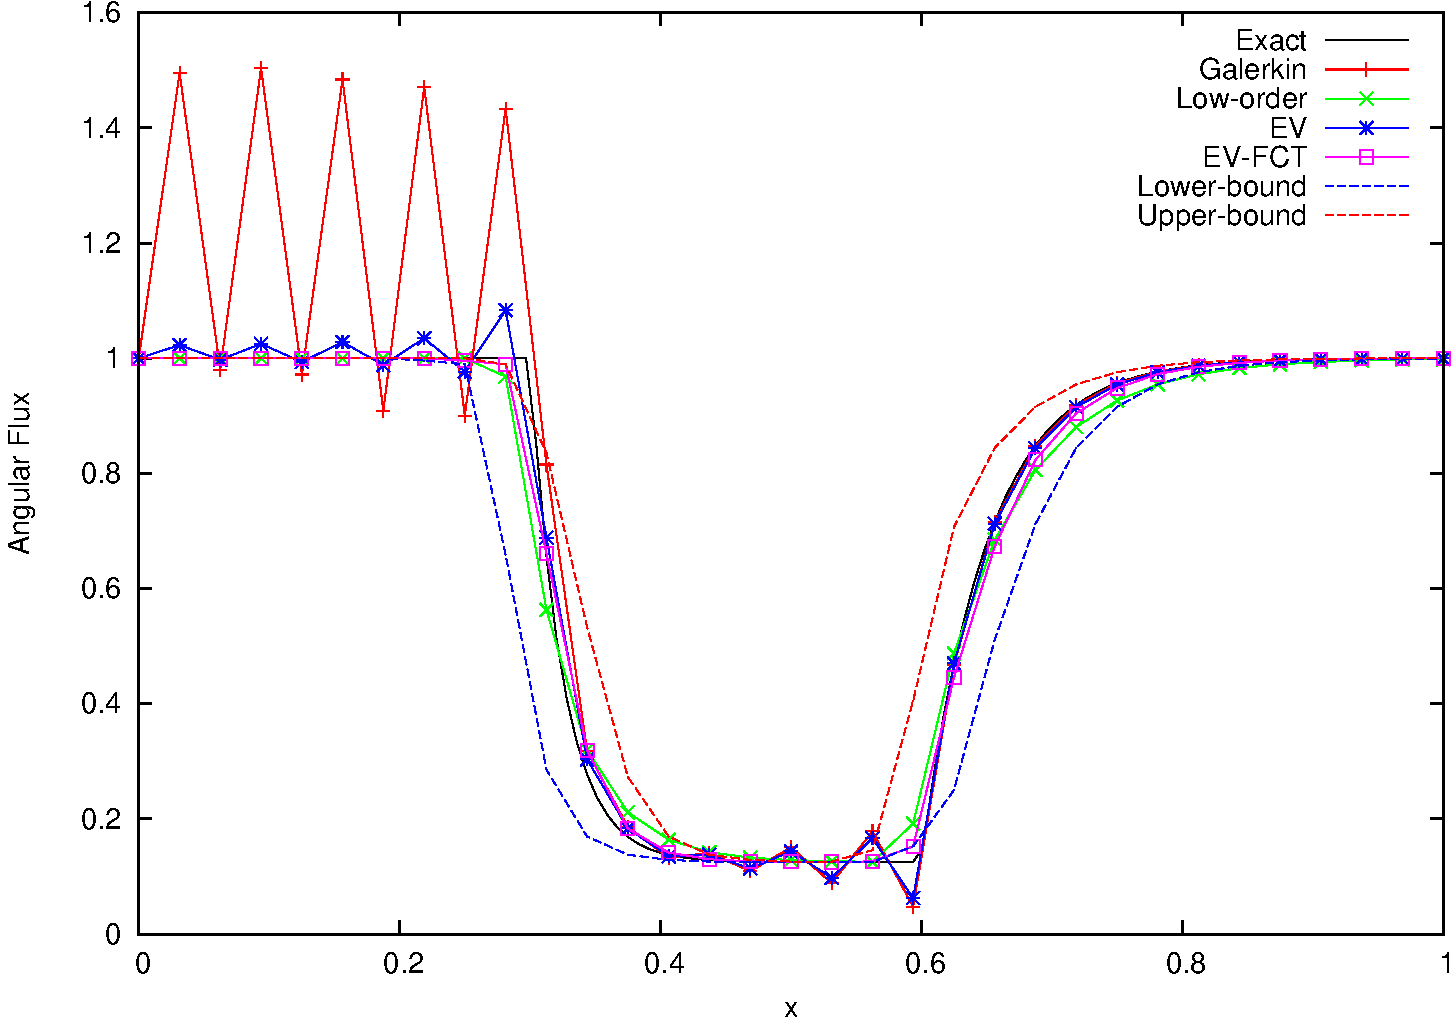
\includegraphics[width=0.9\textwidth]
     {\contentdir/results/transport/three_region/angularflux_SSP3_dmp.pdf}
   \caption{Comparison of Solutions for the 3-Region Test Problem Using SSPRK33
     and DMP Solution Bounds}
   \label{fig:three_region_dmp}
\end{figure}
%-------------------------------------------------------------------------------
%-------------------------------------------------------------------------------
\begin{figure}[ht]
   \centering
   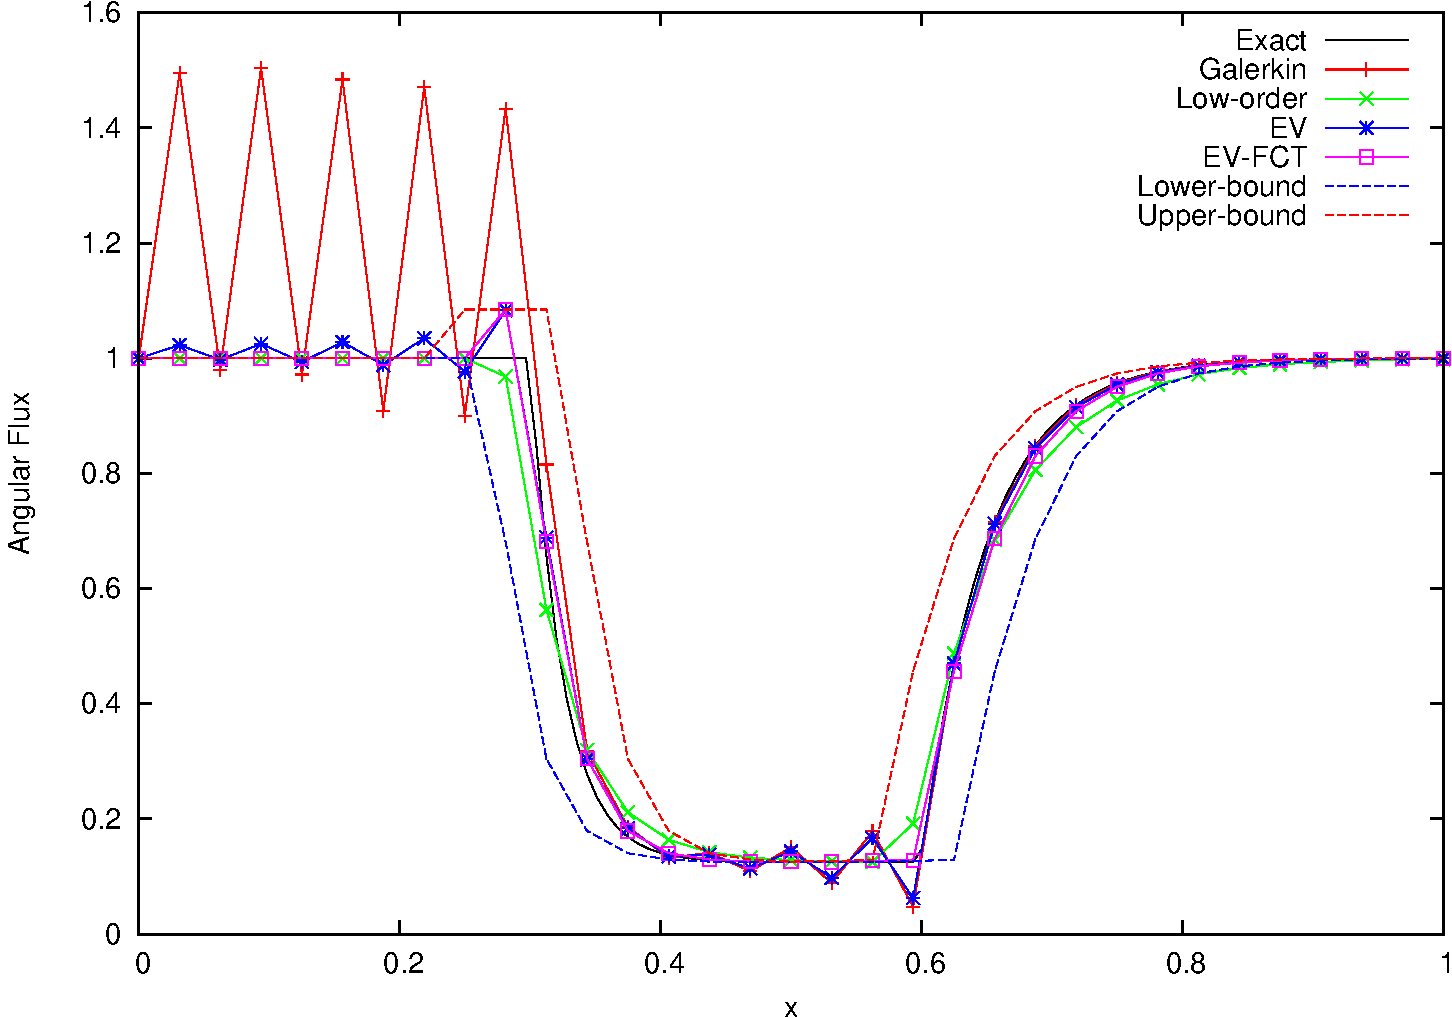
\includegraphics[width=0.9\textwidth]
     {\contentdir/results/transport/three_region/angularflux_SSP3_analytic.pdf}
   \caption{Comparison of Solutions for the 3-Region Test Problem Using SSPRK33
     and Analytic Solution Bounds}
   \label{fig:three_region_analytic}
\end{figure}
%-------------------------------------------------------------------------------
%-------------------------------------------------------------------------------
\begin{figure}[ht]
   \centering
   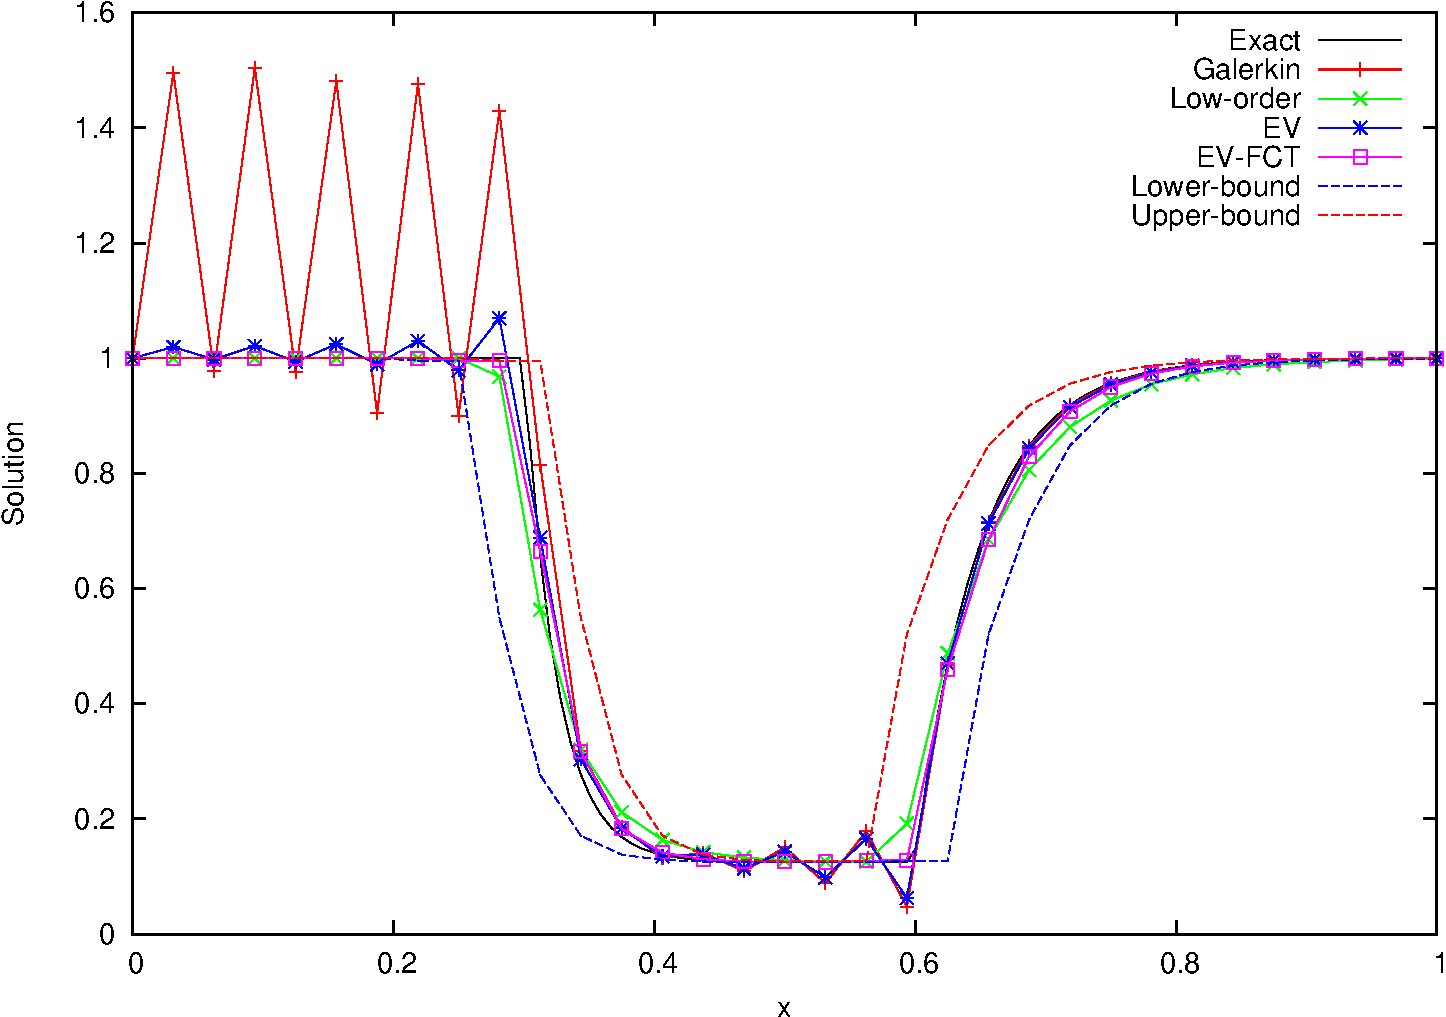
\includegraphics[width=0.9\textwidth]
     {\contentdir/results/transport/three_region/angularflux_SSP3_modified_analytic.pdf}
   \caption{Comparison of Solutions for the 3-Region Test Problem Using SSPRK33
     and Modified Analytic Solution Bounds}
   \label{fig:three_region_modified_analytic}
\end{figure}
%-------------------------------------------------------------------------------
%-------------------------------------------------------------------------------
\begin{figure}[ht]
   \centering
   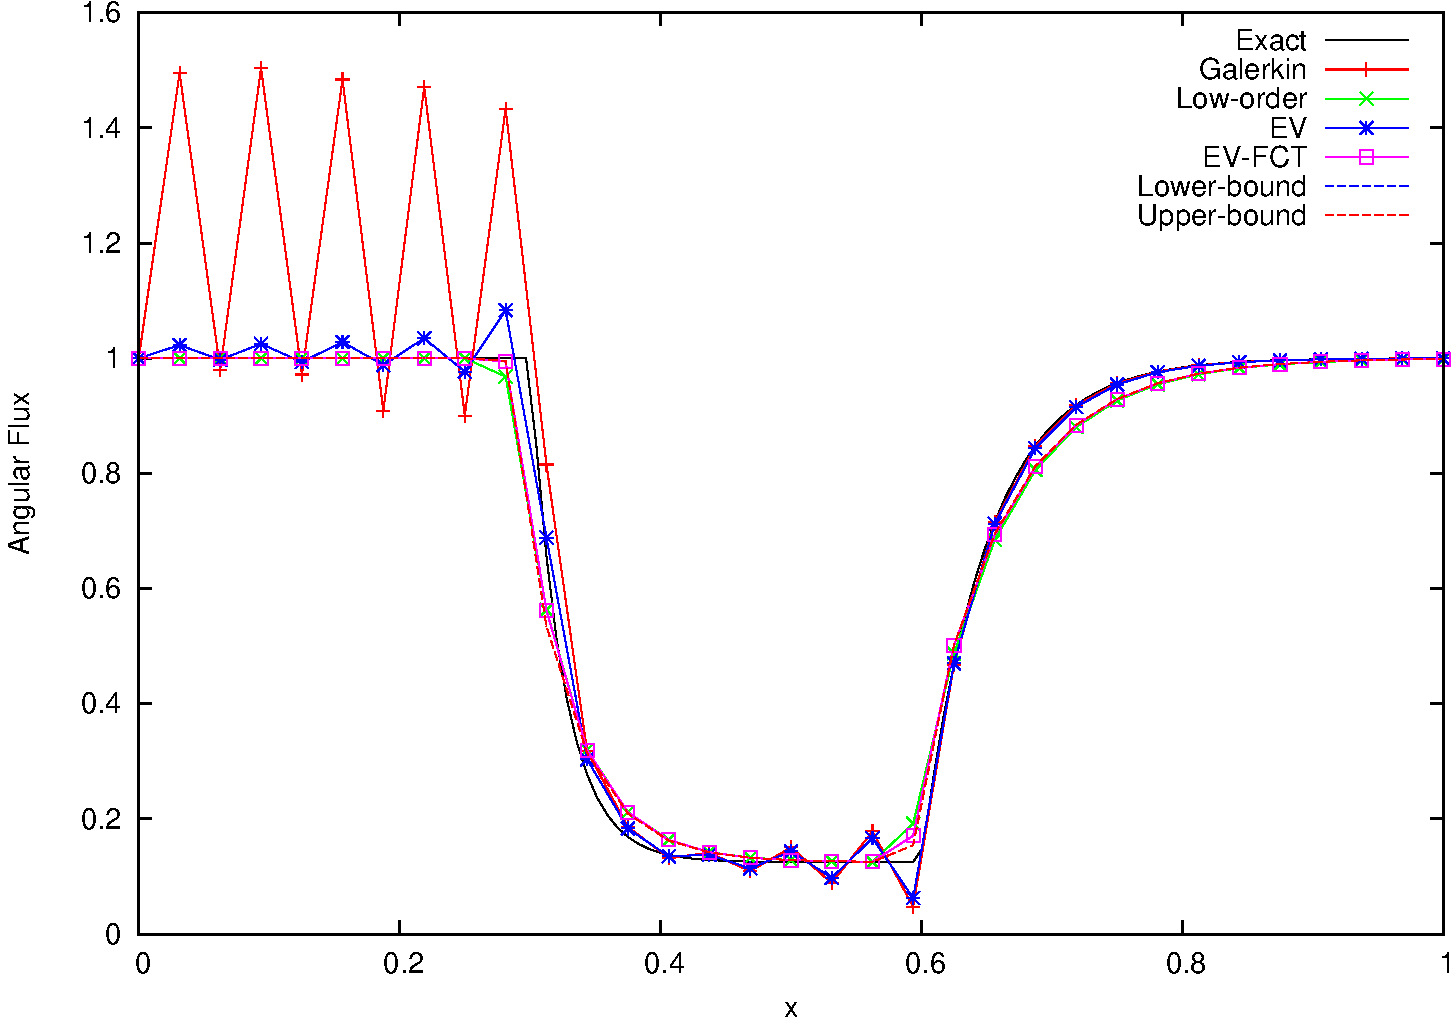
\includegraphics[width=0.9\textwidth]
     {\contentdir/results/transport/three_region/angularflux_SSP3_upwind.pdf}
   \caption{Comparison of Solutions for the 3-Region Test Problem Using SSPRK33
     and Upwind Analytic Solution Bounds}
   \label{fig:three_region_upwind}
\end{figure}
%-------------------------------------------------------------------------------

\clearpage
